% !TeX spellcheck = it_IT
% !TeX document-id = {a2e66a33-fc39-4f27-b56c-a5623f31d5a7}
% !TeX TXS-program:compile = txs:///pdflatex/[--shell-escape]

\documentclass[11pt]{beamer}
\usepackage[utf8]{inputenc}
\usepackage[italian]{babel}
\usepackage{amsmath}
\usepackage{amsfonts}
\usepackage{amssymb}
\usepackage{xmpmulti}
\usepackage{graphicx}
\usepackage{minted}
\usetheme{Berlin} %Malmoe

\beamertemplatenavigationsymbolsempty

\begin{document}
	\author{Federico Pasqua}
	\title{Conway's Game of Life}
	\subtitle{C++, Python e Cython per un Automa Cellulare}
	%\logo{}
	\institute{Università di Pavia}
	%\date{}
	%\subject{}
	%\setbeamercovered{transparent}
	%\setbeamertemplate{navigation symbols}{}
	\begin{frame}[plain]
	\maketitle
\end{frame}

\begin{frame}
\frametitle{Introduzione}
Lo scopo è creare una simulazione di un \emph{Automa Cellulare} del tipo "Conway's Game of Life" che verrà illustrato dopo.\\
Inoltre verrà scritto un motore di simulazione in C++ per poi interfacciarlo ad un applicativo in Python 3 per la parte grafica e di gestione simulazione.\\
Per questo progetto ho ricorso a ben 3 differenti linguaggi di programmazione: C++, Python 3 e Cython per interconnettere i precedenti due.
\end{frame}

\begin{frame}[fragile]{Il Gioco della Vita(?)}
\pause
	\begin{columns}[T] % align columns
		\begin{column}{.48\textwidth}
			\transduration<0-29>{0}
			\multiinclude[<+->][format=png, graphics={width=\linewidth}]{./convert/tmp}
		\end{column}%
		\hfill%
		\begin{column}{.48\textwidth}
			\pause
			Una griglia infinita i cui quadrati possono assumere come valori solo 1 (vivo) o 0 (morto).\\
			Ogni cella viene chiamata "cellula" ed è l'unità fondamentale del gioco. Il tempo è discretizzato e quindi si misura in "generazioni".\\
			Ad ogni generazione avviene un elaborazione che porta all'evoluzione del sistema in uno stato differente.
		\end{column}%
	\end{columns}
\end{frame}
\begin{frame}{Game of Life - The Rule}
\begin{columns}[T] % align columns
	\begin{column}{.48\textwidth}
		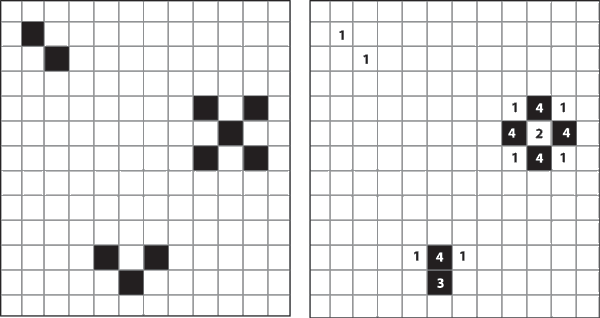
\includegraphics[width=\linewidth]{ExampleRule.png}
	\end{column}%
	\hfill%
	\begin{column}{.48\textwidth}
		Il modo in cui avanza la simulazione da una generazione all'altra si incarna in una \textit{\textbf{Rule}}.\\
		La Regola ci dice da una generazione alla successiva con quante cellule vive confinanti deve stare una cellula morta per "resuscitare" e tornare 1, oltre che quante devono stare vicino ad una cellula già viva affinché non "muoia" e torni 0.
	\end{column}%
\end{columns}
\end{frame}
\begin{frame}
\begin{center}
	\huge Il Game of Life è solo questo.
\end{center}
\normalsize Inoltre, la regola di Conway è detta \textbf{B3/S23}.\\
Ovvero che una cellula morta per tornare viva (Birth) deve avere 3 cellule vive vicino alla generazione precedente, mentre una cellula già viva per restarlo (Stay) deve avere o 2 o 3 cellule vive vicine alla generazione precedente.\\\\
Questa sarà la regola che utilizzeremo nella nostra simulazione, ma lasciando spazio ad un possibile futuro cambiamento.
\end{frame}

\begin{frame}
\frametitle{Obiettivi - Riassunto}
\begin{itemize}
	\pause
	\item \textbf{Libreria di simulazione per il Game of Life} \\
	Questo è l'obiettivo primario. Verrà scritta in C++ per avere una buona performance e usando paradigma OOP.
	\pause
	\item \textbf{Interfaccia tra la libreria C++ e Python} \\
	Questo è il punto critico. Utilizzando una versione espansa del Python detta Cython, verrà creata un interfaccia Python per la libreria, senza necessità di riscriverla.
	\pause
	\item \textbf{Applicazione grafica interattiva} \\
	Questo obiettivo è il motivo per cui si è passati ad un approccio ibrido al problema, spacchettandolo e risolvendolo con ben 3 strumenti differenti. Sarà interattivo, con GUI non testuale e adattabile. Sfruttera le peculiarità del Python.
\end{itemize}
\end{frame}

\begin{frame}
\frametitle{Perché il C++?}
\begin{itemize}
	\pause
	\item \textbf{Tipizzazione Statica}\\
	Ogni variabile in C++ ha un tipo ad essa assegnata. Questo riduce il tempo di esecuzione del programma riducendo di molto l'overhead\footnotemark subito dal programma finale in esecuzione.
	\pause
	\item \textbf{Linguaggio Compilato} \\
	Questo permette di rimuovere determinati errori già in fase di compilazione rendendo intrinsecamente più sicuro il linguaggio. Inoltre la velocità del codice finale è massima.
	\pause
	\item \textbf{VELOCE!} \\
	Grazie ai precedenti due punti abbiamo infine un linguaggio che produce applicativi veloci e ottimizzati sotto ogni punto di vista, grazie anche a GCC e ai suoi 30 anni di esperienza.\footnotemark
\end{itemize}
\footnotetext[1]{Tempo impiegato per l'accesso all'esecuzione di risorse accessorie.}
\footnotetext[2]{First Release: 23 Maggio 1987; C++ Release: Dicembre 1987}
\end{frame}

\begin{frame}
\frametitle{Perché NON il C++?}
\begin{itemize}
	\pause
	\item \textbf{GUI non standard}\\
	Non esiste nessuna libreria GUI standard, costringendo l'uso di librerie terze parti come grafica. Solo di recente la libreria \texttt{Boost} ha proposto un prototipo di standard per l'UI.\footnotemark
	\pause
	\item \textbf{Curva d'apprendimento ripida} \\
	L'impegno richiesto per impararne le funzionalità di livello medio o più è enorme, richiedendo anni anche solo ad imparare a usare un costrutto decentemente.
	\pause
	\item \textbf{LENTO nello sviluppo!} \\
	Scrivere un programma, proprio a causa della sete di specifiche del linguaggio stesso, richiede impegno e soprattutto tempo. Non puoi scrivere C++ o impararlo velocemente.
\end{itemize}
\footnotetext{Boost.UI - https://github.com/kosenko/ui - pubblicata il 26/09/2017}
\end{frame}

\begin{frame}
\frametitle{Cosa c'entra Python?}
\begin{columns}[T] % align columns
	\begin{column}{.48\textwidth}
		
\includegraphics[width=\linewidth]{C_Python.JPG}
	\end{column}%
	\hfill%
	\begin{column}{.48\textwidth}
		Il Python ha caratteristiche diametralmente opposte al C++.\\
		Questo è dovuto anche ad un differente approccio al programma tra i due linguaggi. Uno preferisce la stabilità e la velocità d'esecuzione, l'altro la maneggevolezza, la velocità di scrittura e la leggibilità.
	\end{column}%
\end{columns}
\end{frame}

\begin{frame}[fragile]{Hello World - C++ vs Python}
\begin{itemize}
	\pause
	\item \textbf{C++}\\
	\begin{minted}{c++}
#include <iostream>
using namespace std;
int main() {
    cout << "Hello World!" << endl;
    return 0;
}
	\end{minted}
	\pause
	\item \textbf{Python 3} \\
	\begin{minted}{python3}
print("Hello World!")
	\end{minted}
\end{itemize}
\end{frame}

\begin{frame}
\frametitle{Perché il Python?}
\begin{itemize}
	\pause
	\item \textbf{"Questo è plagio! Usi solo librerie esterne!"}\\
	Python è famoso per avere un quantità di moduli incredibile\footnotemark, ed anche per l'esistenza di moduli particolarmente ottimizzati in grado di fare praticamente qualunque cosa si desideri.
	\pause
	\item \textbf{VELOCE nello sviluppo} \\
	Ottimo per scrivere programmi in poco tempo, dato che l'intero linguaggio è stato disegnato per essere utile, veloce da usare e maneggevole più di ogni altra cosa.
	\pause
	\item \textbf{I moduli di grafica sono semplici} \\
	Molti moduli di grafica disponibili per Python sono facili da usare o comunque molto più semplici della media di difficoltà delle librerie C++.
\end{itemize}
\footnotetext{Al 5 Novembre 2017 la repository ufficiale \texttt{PyPI} contiene 121006 moduli}
\end{frame}

\begin{frame}{Python + C++ = ?}
Ma con tutte queste differenze come faccio a collegare questi due mondi così diversi?\\\\
\pause
Python ha una API, una libreria chiamata C-API, che permette al Python di essere interagibile da un programma in C++.\\
Però questa libreria per C++ è particolarmente ostica e difficile da usare.
\end{frame}

\begin{frame}
\frametitle{Cython}
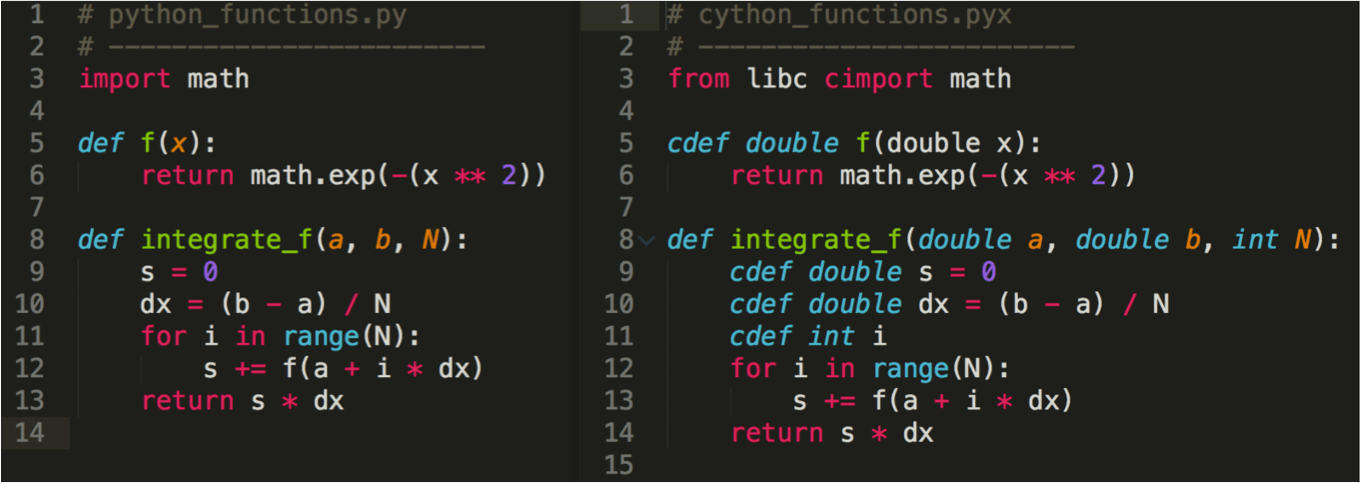
\includegraphics[width=\linewidth]{cython-code.png}
Cython è un superset del linguaggio Python. Esso va a compensare la più grande mancanza di Python, ovvero la velocità. \\
Oltre a questo è anche in grado di fornire i pro del C++ e anche di interconnettere facilmente i due environment.
\end{frame}

\begin{frame}
\frametitle{Cython: Pro e Contro}
\begin{columns}[T] % align columns
	\pause
	\begin{column}{.48\textwidth}
		\textbf{Pro:}
		\begin{itemize}
			\item \textbf{La sintassi di base è quella di Python.}
			\item \textbf{Velocità di esecuzione del C++.}
			\item \textbf{Compila in dynamic link libraries (DLL).}
			Un compilato può essere importato da qualunque istanza Python.
			\item \textbf{Può accedere a codice C/C++.}
		\end{itemize}
	\end{column}%
	\hfill%
	\begin{column}{.48\textwidth}
		\pause
		\textbf{Contro:}
		\begin{itemize}
			\item \textbf{Convertire librerie C++ in moduli Python non è automatico.}
			Viene richiesto infatti un minimo di lavoro manuale.
			\item \textbf{Non rimpiazza C/C++.}
			Cython è comunque Python. Ad esempio non potrei mai scrivere un kernel in Cython.
		\end{itemize}
	\end{column}
\end{columns}
\end{frame}

\begin{frame}
\frametitle{Architettura}
\centering
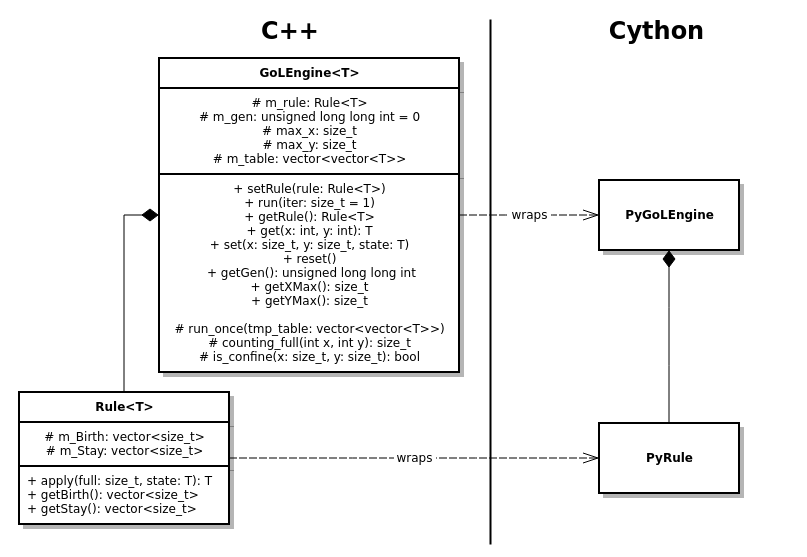
\includegraphics[width=0.92\linewidth]{UML1.png}
\end{frame}

\begin{frame}
Con questa divisione dei compiti mi ritrovo con tutta la parte numerica della simulazione eseguita da un codice in C++ naturalmente ottimizzato e veloce e dei wrapper pronti per l'utilizzo in Python.\\\\
Successivamente da Python verranno dati i parametri della simulazione.\\\\
Fare l'intera simulazione in C++ avrebbe dato una velocità imbattibile, ma il tempo necessario alla sua realizzazione sarebbe stato eccessivo visto anche l'obiettivo di poter facilmente interfacciare una GUI alla simulazione
\end{frame}

\begin{frame}
\frametitle{Tour del Codice}
Ora illustrerò il codice.\\\\
Non utilizzerò le slide data la difficoltà di condensare \textit{"le cose giuste"} nelle sole slide.
\end{frame}

\begin{frame}
\frametitle{Esempi Python + C++ nel mondo reale}
\begin{itemize}
	\pause
	\item \textbf{SciPy ecosystem}
	Ecosistema di moduli Python (\texttt{NumPy}, \texttt{SciPy}, \texttt{MatPlotLib}, \texttt{Pandas} e \texttt{SymPy}) per il calcolo numerico, scientifico, simbolico e la manipolazione e visualizzazione di dati.
	\pause
	\item \textbf{Scikit-learn}
	Modulo di Machine Learning per Python. Implementata quasi interamente in Cython per il bisogno di velocità nel calcolo statistico.
	\pause
	\item \textbf{Quora}
	Piattaforma di domande e risposte con un certo livello di contenuto. Scritto interamente in Python, ha portato i bottleneck in Cython.
	\pause
	\item \textbf{Tensorflow}
	Enorme libreria di machine learning e reti neurali mantenuta da Google. Scritta in C++ e wrappata avendo come bersaglio Python. Sono disponibili anche API per altri linguaggi quali appunto C++, Java e Go.
\end{itemize}
\end{frame}

\begin{frame}
\centering
\Huge Grazie dell'attenzione
\end{frame}

\end{document}